\documentclass[b5paper]{standalone}
\usepackage{fontspec}
\usepackage{polyglossia}
\usepackage{tikz}
\usepackage{ifthen}   
\usepackage{amsmath}
\usepackage{graphics}
\usetikzlibrary{calc}
%
\setmainlanguage{english}
\setotherlanguages{arabic}
\newfontfamily\arabicfont[Scale=1.0,Script=Arabic]{Scheherazade}
\newfontfamily\urdufont[Scale=1.0,Script=Arabic]{XB Tabriz}

\begin{document}
\begin{urdufont}
\begin{tikzpicture}
    \node[anchor=south west,inner sep=0] (image) at (0,0) {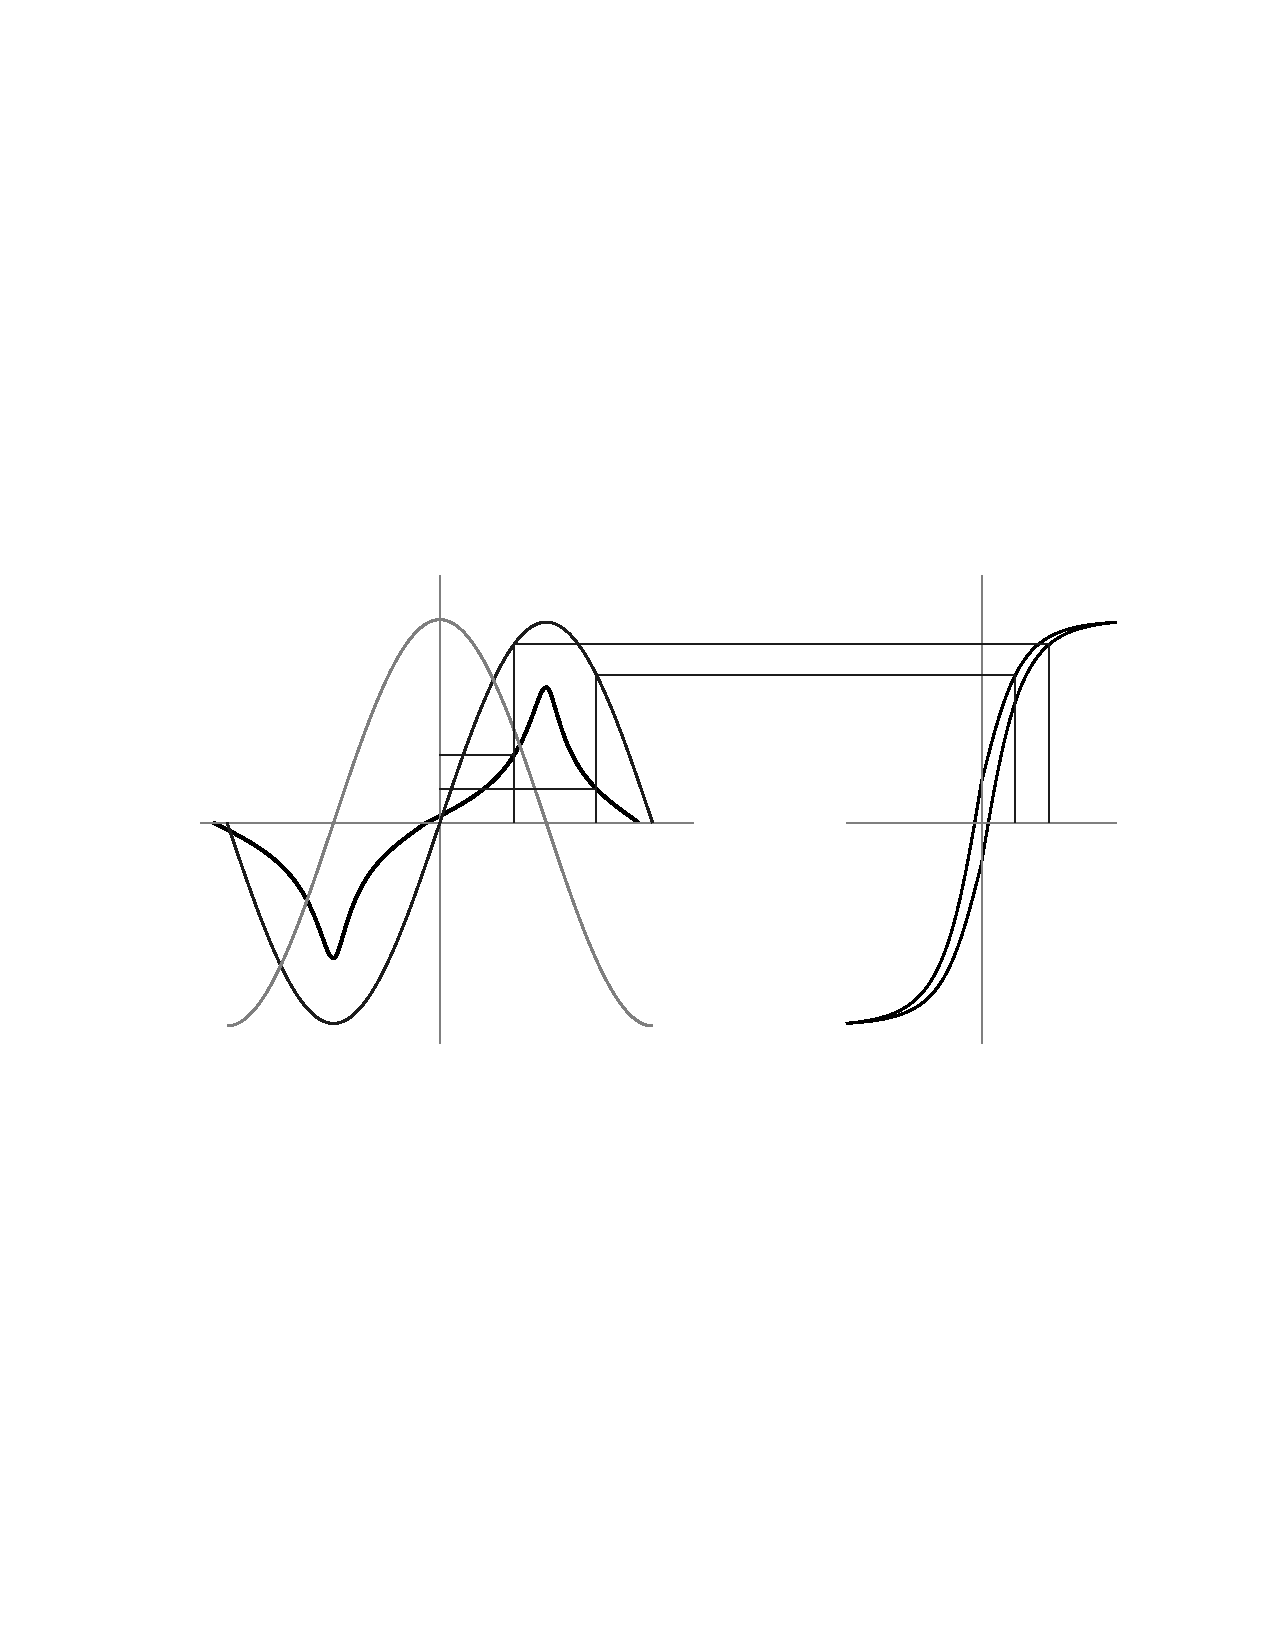
\includegraphics[width=0.9\textwidth,trim={1.5cm 10cm 1cm 9.6cm},clip]{figExcitationCurrentFromBHbrillouinCurve}};
    \begin{scope}[x={(image.south east)},y={(image.north west)}]
%grid
%\draw [gray, thick,xstep=0.1,ystep=0.1] (0,0) grid (1,1);
%\draw [gray, thin,xstep=0.01,ystep=0.01] (0,0) grid (1,1);

\node at (0.376,0.44){$t_1$};
\node at (0.45,0.44){$t_2$};
\node[gray] at (0.55,0.44){$t$};
\node at (0.86,0.44){$i_1$};
\node at (0.825,0.44){$i_2$};
\node[gray] at (0.94,0.44){$i_\varphi$};
\node at (0.29,0.64){$i_1$};
\node at (0.29,0.56){$i_2$};
\node[gray] at (0.29,0.98){$i_\varphi$};
\node[fill=white] at (0.15,0.3){$\varphi$};
\node[fill=white] at (0.25,0.4){$i_\varphi$};
\node[gray,fill=white] at (0.25,0.7){$e$};

\node[gray] at (0.77,0.95){$\varphi$};
\node at (0.36,0.88){$\varphi_1$};
\node at (0.485,0.74){$\varphi_2$};

\node at (0.9,0.1){الف};
\node at (0.4,0.1){ب};

    \end{scope}
\end{tikzpicture}
\end{urdufont}
\end{document}

